\section{TA Evaluation UI Improvements}

Two static panels have been added which contains the navigation and download options which are essential and frequently used during evalution by the TAs and the instructor. These panels have been optimally designed to occupy minimum space so as to not interfere with the viewability of the answer sheet, as well to provide maximum usability.

\subsection{Navigation Panel}
The navigation panel contains \textbf{Next} and \textbf{Previous} buttons which can be used by the TAs for easily navigation to other submissions. A \textbf{Download submitted files} button is also present in the panel, which when clicked downloads the files submitted as part of the current answer sheet. This is much better than the earlier ``Search for student files'' interface. This is shown in figure \ref{fig:nav_panel}.

\begin{figure}[H]

\includegraphics[width=\textwidth]{images/nav_panel}
\caption{Navigation Panel}
\label{fig:nav_panel}
\end{figure}

\subsection{Question Index Panel}
A static index panel has been added to the answer sheet that lists the question numbers. Clicking on a question number scrolls to that question directly, so the TA doesn't have do it manually.\\
The question numbers are colour-coded which shows the status of its evaluation. Green denotes evaluated and Red means the question is yet to be evaluated. A sample is shown in figure \ref{fig:index_panel}.

\begin{figure}[H]
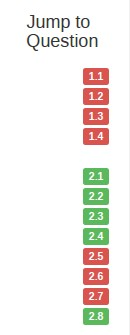
\includegraphics{images/index_panel}
\caption{Index Panel}
\label{fig:index_panel}
\end{figure}

\subsection{Auto-evaluate unattempted questions}
Marks for those questions which are not answered are automatically set as zero. Also, the evaluation status of such questions in the Question Index Panel is set as `evaluated' so that the TAs need not check them at all.

\subsection{Remove alert boxes}
Both in student interface while answering the paper, and TA interface while evaluating (adding comments), javascript alert boxes were popping up. This feature which required a user interaction (mouse-click) was removed, and instead a notification message is shown which disappears automatically.
